% ============================================================
%  AlphaStream India -- Primary Submission Document
%  ET AI Hackathon 2026 -- Problem Statement 6
%  "AI for the Indian Investor"
% ============================================================
\documentclass[11pt, a4paper]{article}

% -- Core packages -----------------------------
\usepackage[a4paper, top=2.2cm, bottom=2.2cm,
            left=2.4cm, right=2.4cm, headheight=14pt]{geometry}
\usepackage[T1]{fontenc}
\usepackage[utf8]{inputenc}
\DeclareUnicodeCharacter{20B9}{\Rs}
\newcommand{\Rs}{Rs.\,}
% -- Fonts: Source family (modern, clean, professional) ------
\usepackage[default]{sourceserifpro}   % Serif body text
\usepackage[scale=0.95]{sourcesanspro} % Sans for headings
\usepackage[scale=0.92]{sourcecodepro} % Mono for code listings
\usepackage{microtype}
\usepackage{parskip}
\usepackage{setspace}
\usepackage{graphicx}

% -- Color ----------------------------------
\usepackage{xcolor}
\definecolor{navy}{RGB}{26,  58, 107}
\definecolor{cyan}{RGB}{ 0, 180, 216}
\definecolor{teal}{RGB}{ 0, 128, 128}
\definecolor{green}{RGB}{45, 156,  77}
\definecolor{orange}{RGB}{230, 126, 34}
\definecolor{purple}{RGB}{142,  68, 173}
\definecolor{red}{RGB}{192,  57,  43}
\definecolor{steel}{RGB}{ 52,  73,  94}
\definecolor{lgray}{RGB}{248, 248, 248}
\definecolor{mgray}{RGB}{170, 170, 170}
\definecolor{gold}{RGB}{241, 196, 15}
\definecolor{darkgreen}{RGB}{39, 174, 96}

% -- TikZ -----------------------------------
\usepackage{tikz}
\usetikzlibrary{
  shapes.geometric, shapes.multipart,
  arrows.meta, positioning, fit,
  backgrounds, calc, shadows.blur,
  decorations.pathmorphing, trees
}

% -- Tables ----------------------------------
\usepackage{booktabs}
\usepackage{tabularx}
\usepackage{longtable}
\usepackage{array}
\usepackage{multirow}
\usepackage{colortbl}

% -- Layout / headings --------------------------
\usepackage{titlesec}
\usepackage{fancyhdr}
\usepackage{float}
\usepackage{caption}
\usepackage{enumitem}
\usepackage{amsmath}
\usepackage{amssymb}
\usepackage{multicol}
\usepackage{wrapfig}

% -- Boxes ----------------------------------
\usepackage{tcolorbox}
\tcbuselibrary{skins, breakable}

% -- Links ----------------------------------
\usepackage[hidelinks, colorlinks=true, linkcolor=navy, urlcolor=cyan!70!black]{hyperref}

% -- Code listings -----------------------------
\usepackage{listings}
\lstset{
  basicstyle=\ttfamily\scriptsize,
  backgroundcolor=\color{lgray},
  frame=single, framerule=0.4pt,
  rulecolor=\color{mgray},
  breaklines=true, breakatwhitespace=true,
  showstringspaces=false,
  keywordstyle=\color{navy}\bfseries,
  commentstyle=\color{mgray},
  stringstyle=\color{teal},
  numbers=left, numberstyle=\tiny\color{mgray},
  numbersep=5pt
}

% ============================================================
%  Section formatting
% ============================================================
\setstretch{1.15}

\titleformat{\section}
  {\Large\bfseries\sffamily\color{navy}}
  {\thesection.}{0.6em}{}
  [\vspace{0pt}\color{cyan}\rule{\linewidth}{1.5pt}\vspace{2pt}]

\titleformat{\subsection}
  {\large\bfseries\sffamily\color{navy!85}}
  {\thesubsection}{0.5em}{}

\titleformat{\subsubsection}
  {\normalsize\bfseries\sffamily\color{navy!70}}
  {\thesubsubsection}{0.5em}{}

\titlespacing{\section}{0pt}{1.2em}{0.5em}
\titlespacing{\subsection}{0pt}{0.9em}{0.35em}
\titlespacing{\subsubsection}{0pt}{0.7em}{0.25em}

% ============================================================
%  Header / footer
% ============================================================
\pagestyle{fancy}
\fancyhf{}
\fancyhead[L]{\small\color{navy}\textbf{AlphaStream India}}
\fancyhead[R]{\small\color{mgray}ET AI Hackathon 2026 \textbar{} PS-6}
\fancyfoot[C]{\small\color{navy}\thepage}
\renewcommand{\headrulewidth}{0.5pt}
\renewcommand{\headrule}{\color{cyan}\hrule width\headwidth height 0.5pt}

% ============================================================
%  tcolorbox styles
% ============================================================
\newtcolorbox{infobox}[1][]{
  enhanced, colback=cyan!6, colframe=cyan!50!navy,
  boxrule=0.7pt, arc=4pt,
  left=7pt, right=7pt, top=5pt, bottom=5pt,
  fonttitle=\bfseries\sffamily\color{white},
  attach boxed title to top left={yshift=-2mm, xshift=4mm},
  boxed title style={colback=cyan!50!navy, arc=3pt, boxrule=0pt},
  #1}

\newtcolorbox{greenbox}[1][]{
  enhanced, colback=green!6, colframe=green!60!black,
  boxrule=0.7pt, arc=4pt,
  left=7pt, right=7pt, top=5pt, bottom=5pt,
  fonttitle=\bfseries\sffamily\color{white},
  attach boxed title to top left={yshift=-2mm, xshift=4mm},
  boxed title style={colback=green!60!black, arc=3pt, boxrule=0pt},
  #1}

\newtcolorbox{orangebox}[1][]{
  enhanced, colback=orange!6, colframe=orange!60!black,
  boxrule=0.7pt, arc=4pt,
  left=7pt, right=7pt, top=5pt, bottom=5pt,
  fonttitle=\bfseries\sffamily\color{white},
  attach boxed title to top left={yshift=-2mm, xshift=4mm},
  boxed title style={colback=orange!60!black, arc=3pt, boxrule=0pt},
  #1}

\newtcolorbox{purplebox}[1][]{
  enhanced, colback=purple!5, colframe=purple!50!navy,
  boxrule=0.7pt, arc=4pt,
  left=7pt, right=7pt, top=5pt, bottom=5pt,
  fonttitle=\bfseries\color{navy!80}, #1}

\newtcolorbox{keymetricbox}{
  enhanced, colback=navy!5, colframe=navy!70,
  boxrule=1pt, arc=6pt,
  left=10pt, right=10pt, top=8pt, bottom=8pt}

% ============================================================
%  Global TikZ style definitions
% ============================================================
\tikzset{
  layerA/.style={draw=steel!70!black, fill=steel!12,
    rounded corners=5pt, minimum width=12.4cm, minimum height=1.5cm,
    text width=12.0cm, align=center, font=\small},
  layerB/.style={draw=navy!70!black, fill=navy!10,
    rounded corners=5pt, minimum width=12.4cm, minimum height=1.5cm,
    text width=12.0cm, align=center, font=\small},
  layerC/.style={draw=purple!60!black, fill=purple!8,
    rounded corners=5pt, minimum width=12.4cm, minimum height=1.5cm,
    text width=12.0cm, align=center, font=\small},
  layerD/.style={draw=green!60!black, fill=green!8,
    rounded corners=5pt, minimum width=12.4cm, minimum height=1.5cm,
    text width=12.0cm, align=center, font=\small},
  layerE/.style={draw=red!60!black, fill=red!8,
    rounded corners=5pt, minimum width=12.4cm, minimum height=1.5cm,
    text width=12.0cm, align=center, font=\small},
  agentbox/.style={draw=navy!55, fill=navy!10,
    rounded corners=3pt, minimum width=2.6cm, minimum height=0.8cm,
    text width=2.4cm, align=center, font=\scriptsize\bfseries},
  decisionbox/.style={draw=green!65!black, fill=green!15,
    rounded corners=5pt, minimum width=4.2cm, minimum height=1.2cm,
    text width=4.0cm, align=center, font=\small\bfseries},
  outputbox/.style={draw=orange!65!black, fill=orange!12,
    rounded corners=4pt, minimum width=3.2cm, minimum height=1.0cm,
    text width=3.0cm, align=center, font=\scriptsize\bfseries},
  groupfit/.style={draw=navy!30, fill=navy!4,
    dashed, rounded corners=6pt, inner sep=6pt},
  nlqnode/.style={draw=navy!60, fill=cyan!12,
    rounded corners=4pt, minimum width=2.0cm, minimum height=0.85cm,
    text width=1.8cm, align=center, font=\scriptsize\bfseries},
  nlqdb/.style={draw=purple!60, fill=purple!10,
    rounded corners=4pt, minimum width=2.0cm, minimum height=0.85cm,
    text width=1.8cm, align=center, font=\scriptsize\bfseries},
  nlqio/.style={draw=green!60!black, fill=green!12,
    rounded corners=4pt, minimum width=2.0cm, minimum height=0.85cm,
    text width=1.8cm, align=center, font=\scriptsize\bfseries},
  mainarrow/.style={->, >=Stealth, line width=1.4pt, color=navy!65},
  subarrow/.style={->, >=Stealth, line width=0.9pt, color=navy!45},
  sidarrow/.style={->, >=Stealth, line width=0.9pt, color=cyan!70!navy, dashed}
}

% ============================================================
%  Helpers
% ============================================================
\newcolumntype{L}[1]{>{\raggedright\arraybackslash}p{#1}}
\newcolumntype{C}[1]{>{\centering\arraybackslash}p{#1}}
\newcolumntype{R}[1]{>{\raggedleft\arraybackslash}p{#1}}

\newcommand{\statbox}[2]{%
  \begin{tcolorbox}[enhanced, colback=navy!6, colframe=navy!40,
    boxrule=0.5pt, arc=4pt, width=3.6cm, height=1.6cm,
    halign=center, valign=center]
    {\Large\bfseries\color{navy}#1}\\[2pt]
    {\scriptsize\color{steel}#2}
  \end{tcolorbox}%
}

% ============================================================
\begin{document}

% -- Title page -------------------------------
\begin{titlepage}
  \centering
  \vspace*{0.8cm}

  {\color{cyan}\rule{\linewidth}{2.5pt}}
  \vspace{0.6cm}

  {\fontsize{32}{38}\selectfont\bfseries\color{navy}
    AlphaStream India}\\[0.5cm]
  {\Large\color{steel}
    Real-Time AI Investment Intelligence\\for the Indian Retail Investor}

  \vspace{0.5cm}
  {\color{cyan}\rule{\linewidth}{2.5pt}}

  \vspace{0.8cm}

  % Key metrics strip
  
\begin{tikzpicture}
    \node[fill=navy!8, rounded corners=6pt, inner sep=10pt, text width=14cm, align=center] {
      \begin{tabular}{ccccc}
        {\Large\bfseries\color{navy}13} & {\Large\bfseries\color{navy}$<$2s} &
        {\Large\bfseries\color{navy}30+} & {\Large\bfseries\color{navy}5} &
        {\Large\bfseries\color{navy}14Cr+} \\
        {\tiny\color{steel}AI Agents} & {\tiny\color{steel}News-to-Signal} &
        {\tiny\color{steel}API Endpoints} & {\tiny\color{steel}Tab Terminal} &
        {\tiny\color{steel}Target Users}
      \end{tabular}
    };
  \end{tikzpicture}

  \vspace{0.7cm}

  % Architecture preview
  \begin{tikzpicture}[scale=0.82]
    \node[layerA] (d) at (0,0) {%
      \textbf{\color{steel!80!black}Layer 1: Indian \& Global Data Sources}\\[2pt]
      NSE API \textbullet{} BSE API \textbullet{} FII/DII (NSDL) \textbullet{} Groww API \textbullet{} ET Markets RSS\\
      WorldMonitor \textbullet{} FRED Macro \textbullet{} CNN Fear \& Greed \textbullet{} NewsAPI};
    \node[layerB, below=0.35cm of d] (p)
      {\textbf{\color{navy}Layer 2: Pathway Streaming Engine}\\[2pt]
       ConnectorSubject \textbullet{} Adaptive RAG \textbullet{} pw.io.subscribe \textbullet{} DocumentStore};
    \node[layerC, below=0.35cm of p] (a)
      {\textbf{\color{purple!80!black}Layer 3: Multi-Agent Reasoning (13 Agents)}\\[2pt]
       Sentiment \textbullet{} Technical \textbullet{} Risk \textbullet{} Pattern \textbullet{} Backtest \textbullet{} Flow \textbullet{}
       Filing \textbullet{} Insider \textbullet{} Anomaly \textbullet{} Search \textbullet{} Chart \textbullet{} Report \textbullet{} Decision};
    \node[layerD, below=0.35cm of a] (db)
      {\textbf{\color{green!60!black}Layer 4: DuckDB Analytics + NLQ Engine}\\[2pt]
       DuckDB \textbullet{} ChromaDB \textbullet{} Text2SQL \textbullet{} LangGraph 8-Node Pipeline \textbullet{} MCP Servers};
    \node[layerE, below=0.35cm of db] (fe)
      {\textbf{\color{red!70!black}Layer 5: Bloomberg-Style React Terminal (5 Tabs)}\\[2pt]
       Overview \textbullet{} Signals \textbullet{} Global Intel \textbullet{} Company \textbullet{} Portfolio};

    \draw[mainarrow] (d.south) -- (p.north);
    \draw[mainarrow] (p.south) -- (a.north);
    \draw[mainarrow] (a.south) -- (db.north);
    \draw[mainarrow] (db.south) -- (fe.north);
  \end{tikzpicture}

  \vspace{0.8cm}
  \begin{tabular}{ll}
    \textbf{\color{navy}Competition:}  & ET AI Hackathon 2026 -- Avataar.ai + Unstop \\[3pt]
    \textbf{\color{navy}Problem:}      & PS-6: AI for the Indian Investor \\[3pt]
    \textbf{\color{navy}Repository:}   & \url{https://github.com/wildcraft958/AlphaStream_India} \\[3pt]
    \textbf{\color{navy}Date:}         & March 2026 \\
  \end{tabular}

  \vfill
  {\color{cyan}\rule{\linewidth}{1.5pt}}
\end{titlepage}

% -- Table of contents --------------------------
\tableofcontents
\newpage

% ============================================================
\section{Executive Summary}
% ============================================================

\begin{infobox}[title={One-Line Pitch}]
\textbf{AlphaStream India} is a Bloomberg-style AI investment terminal that transforms
ET Markets data into actionable, real-time, backtested signals for India's
\textbf{14 crore+} retail investors -- replacing 2+ hours of daily research with
AI-powered intelligence delivered in under 2 seconds.
\end{infobox}

\medskip

India has over \textbf{14 crore demat accounts} (CDSL + NSDL, 2024), yet the vast majority
of retail investors are flying blind -- reacting to WhatsApp tips, unable to read technicals,
missing corporate filings, and managing portfolios on gut feel. Institutional investors use
Bloomberg terminals costing \$25,000/year. AlphaStream India bridges this gap with a
\textbf{free, production-grade} alternative built on cutting-edge AI.

\subsection*{What We Built}

\begin{itemize}[leftmargin=1.6em, itemsep=3pt]
  \item \textbf{Opportunity Radar} -- continuously monitors corporate filings, insider trades,
        bulk/block deals, FII/DII flows, and regulatory changes. Surfaces missed opportunities
        as daily alerts with Alpha Scores (0--100). Not a summarizer -- a \emph{signal finder}.
  \item \textbf{Chart Pattern Intelligence} -- real-time detection of breakouts, RSI divergences,
        MACD crossovers, Bollinger breakouts, golden/death crosses across the entire Nifty 50
        universe. Every pattern is backtested over 5 years with verifiable win rates.
  \item \textbf{Market ChatGPT -- Next Gen} -- deeper data integration via Text2SQL against
        a live DuckDB analytics database. Portfolio-aware, multi-step analysis, source-cited
        responses. Answers grounded in \emph{real data}, not LLM hallucination.
  \item \textbf{WorldMonitor Global Intelligence} -- live global indices, crypto, commodities,
        FX, Fear \& Greed, macro signals, and geopolitical risk -- all wired into every
        recommendation with India-specific impact analysis.
\end{itemize}

\subsection*{Key Differentiators}

\begin{center}
\small
\begin{tabular}{L{5.2cm} L{7.8cm}}
  \toprule
  \textbf{What 99\% of Teams Build} & \textbf{What AlphaStream Builds} \\
  \midrule
  Call GPT-4 $\to$ get text blob & Text2SQL pipeline $\to$ grounded in live DuckDB data \\
  No verification of claims & Historical 5-year backtest with verifiable win rates \\
  Mock or delayed data & Live NSE / BSE / FII / NSDL data feeds \\
  Streamlit prototype & Production React 19 + WebSocket + SSE terminal \\
  Single ticker lookup & 13-agent Alpha Score fusion across all Nifty 50 \\
  No guardrails & Input/output guardrails + SQL correction loop \\
  Generic global tickers & India-first: \Rs{}, IST, NSE/BSE, FII/DII, BSE filings \\
  Batch processing & Pathway streaming: news to signal in $<$2 seconds \\
  \bottomrule
\end{tabular}
\end{center}

\begin{greenbox}[title={Submission Artefacts}]
\small
\begin{tabular}{@{}L{4cm}L{9.5cm}@{}}
  \textbf{GitHub Repository}    & \url{https://github.com/wildcraft958/AlphaStream_India} \\
  \textbf{Architecture Doc}     & Separate PDF: Architecture + Impact Model \\
  \textbf{Impact Model}         & Section~\ref{sec:impact} of this document + separate PDF \\
  \textbf{Demo Video}           & 3-minute walkthrough (see script in \texttt{docs/}) \\
\end{tabular}
\end{greenbox}

% ============================================================
\section{Problem Statement}
% ============================================================

\subsection{The Scale of the Problem}

\begin{keymetricbox}
\centering
\begin{tabular}{ccccc}
  {\LARGE\bfseries\color{navy}14 Cr+} &
  {\LARGE\bfseries\color{red}80\%} &
  {\LARGE\bfseries\color{orange}2+ hrs} &
  {\LARGE\bfseries\color{purple}\Rs{}10K} &
  {\LARGE\bfseries\color{steel}0} \\[3pt]
  {\scriptsize\color{steel}Demat Accounts} &
  {\scriptsize\color{steel}Rely on Tips} &
  {\scriptsize\color{steel}Daily Research} &
  {\scriptsize\color{steel}Missed/Quarter} &
  {\scriptsize\color{steel}Free AI Terminals}
\end{tabular}
\end{keymetricbox}

\medskip

India has \textbf{14 crore+ demat accounts} yet the tools available to retail investors
are dramatically inferior to institutional systems:

\begin{itemize}[leftmargin=1.6em, itemsep=3pt]
  \item \textbf{Stale data} -- most free platforms update prices every 5--15 minutes;
        institutional desks consume tick data in real time.
  \item \textbf{No signal aggregation} -- a retail investor checks RSI on one screen, reads
        FII data on NSDL's PDF portal, hunts for insider trades on NSE's filing search --
        three separate workflows with zero synthesis.
  \item \textbf{LLM tools are ungrounded} -- existing ``AI chatbots'' for investing answer
        questions from trained weights, not live market data. They hallucinate stock prices
        and miss earnings announced an hour ago.
  \item \textbf{2+ hours of daily research} -- active retail investors spend 2--3 hours/day
        on research that could be automated, translating to \textbf{\Rs{}2.19 Lakh/year} in
        lost productivity per user.
  \item \textbf{No free alternative to Bloomberg} -- institutional terminals cost \$25,000+/year.
        Retail investors have nothing comparable.
\end{itemize}

\subsection{Our Solution: Live AI}

AlphaStream implements the \textbf{``Live AI'' paradigm} -- a system that continuously ingests data,
updates its knowledge base incrementally (not batch), delivers recommendations reflecting the
current state of reality, and provides full explainability for every decision.

\begin{center}
\small
\begin{tabular}{L{5.5cm} L{7cm}}
  \toprule
  \textbf{Traditional AI Tool} & \textbf{AlphaStream India} \\
  \midrule
  Call GPT-4 $\to$ text blob & Text2SQL $\to$ grounded DuckDB answer \\
  No verification & Historical backtest with win rates \\
  Mock / delayed data & Live NSE / BSE / FII data \\
  Streamlit dashboard & Production React + WebSocket \\
  Single ticker lookup & 13-signal Alpha Score fusion \\
  No guardrails & Input/output guardrails + SQL correction loop \\
  Generic (global tickers) & India-first (NSE/BSE, \Rs{}, IST, FII/DII) \\
  \bottomrule
\end{tabular}
\end{center}

% ============================================================
\section{System Architecture}
\label{sec:arch}
% ============================================================

\subsection{Five-Layer Architecture}

The system is organized into five vertically-stacked layers, each communicating
with the next via well-defined interfaces: REST calls, Pathway streaming callbacks,
WebSocket events, and DuckDB SQL queries.

\begin{figure}[H]
\centering
\begin{tikzpicture}[node distance=0.45cm]

  \node[layerA] (datasrc)
    {\textbf{\color{steel!80!black}Layer 1 -- Indian \& Global Data Sources}\\[3pt]
     \small NSE OHLCV \quad BSE Announcements \quad
     FII/DII Flows (NSDL) \quad Groww Fundamentals\\
     ET Markets RSS \quad WorldMonitor (yfinance) \quad
     FRED Macro \quad CNN Fear \& Greed \quad NewsAPI};

  \node[layerB, below=0.45cm of datasrc] (pathway)
    {\textbf{\color{navy}Layer 2 -- Pathway Streaming Engine}\\[3pt]
     \small pw.io.python.ConnectorSubject \quad Adaptive RAG (xpacks.llm) \quad
     DocumentStore \quad pw.io.subscribe\\
     UsearchKnnFactory (vector index) \quad pw.run (background daemon) \quad
     pw.io.fs.read (article cache)};

  \node[layerC, below=0.45cm of pathway] (agents)
    {\textbf{\color{purple!80!black}Layer 3 -- Multi-Agent Reasoning (13 Agents)}\\[3pt]
     \small Sentiment \textbullet{} Technical \textbullet{} Risk \textbullet{} Pattern \textbullet{}
     Backtest \textbullet{} Flow \textbullet{} Filing \textbullet{}
     Insider \textbullet{} Anomaly \textbullet{} Search \textbullet{} Chart \textbullet{}
     Report \textbullet{} Decision\\
     \textit{All agents use Gemini 2.0 Flash (Vertex AI) via LangChain}};

  \node[layerD, below=0.45cm of agents] (analytics)
    {\textbf{\color{green!60!black}Layer 4 -- Analytics \& NLQ Engine}\\[3pt]
     \small DuckDB (\texttt{market\_analytics.duckdb}) \quad
     fact\_articles \textbullet{} fact\_signals \textbullet{} fact\_insider\_trades \textbullet{}
     fact\_fii\_dii\_flows \textbullet{} dim\_stocks\\
     Views: v\_stock\_screener \textbullet{} v\_signal\_summary \textbullet{}
     v\_sector\_heatmap \quad ChromaDB (vector store)};

  \node[layerE, below=0.45cm of analytics] (frontend)
    {\textbf{\color{red!70!black}Layer 5 -- React Terminal + API Layer}\\[3pt]
     \small LangGraph 8-node NLQ (Text2SQL + Guardrails) \quad
     FastAPI REST (30+ endpoints) \quad WebSocket \quad SSE\\
     React 19 + Tailwind + Recharts + Lightweight-Charts
     \quad Bloomberg-style 5-tab terminal};

  \draw[mainarrow] (datasrc.south) -- (pathway.north);
  \draw[mainarrow] (pathway.south) -- (agents.north);
  \draw[mainarrow] (agents.south) -- (analytics.north);
  \draw[mainarrow] (analytics.south) -- (frontend.north);

  \node[right=0.4cm of datasrc,  align=left, font=\tiny\color{mgray}]
    {Real-time\\ingestion};
  \node[right=0.4cm of pathway,  align=left, font=\tiny\color{mgray}]
    {Streaming\\callbacks};
  \node[right=0.4cm of agents,   align=left, font=\tiny\color{mgray}]
    {Signal\\fusion};
  \node[right=0.4cm of analytics, align=left, font=\tiny\color{mgray}]
    {SQL\\queries};

\end{tikzpicture}
\caption{AlphaStream India -- Five-Layer System Architecture}
\end{figure}

\subsection{End-to-End Data Flow}

\begin{enumerate}[leftmargin=1.8em, itemsep=3pt]
  \item \textbf{Ingest}: The Pathway \texttt{ConnectorSubject} polls 5 news APIs in
        parallel every 60 seconds; articles are written to \texttt{data/articles/}.
        NSE/BSE connectors fetch OHLCV, filings, and insider trades.
  \item \textbf{Index}: \texttt{pw.io.fs.read} detects new files and the
        \texttt{DocumentStore} chunks, embeds (all-MiniLM-L6-v2), and indexes them
        into UsearchKnnFactory -- all incrementally, with no full rebuild.
  \item \textbf{Callback}: \texttt{pw.io.subscribe} fires \texttt{on\_new\_article()}
        on each new row, triggering DuckDB persistence and WebSocket broadcasts.
  \item \textbf{Reason}: On a \texttt{POST /recommend} request, 13 specialist agents
        run in parallel (via \texttt{asyncio.gather}). The FusionEngine combines scores
        with configurable weights into a single Alpha Score (0--100).
  \item \textbf{Deliver}: The response is pushed to the React dashboard over
        WebSocket (\texttt{/ws/stream/\{ticker\}}) in under 50\,ms.
\end{enumerate}

\subsection{DuckDB Analytics Schema}

The analytics layer uses a star schema optimized for fast aggregation:

\begin{center}
\small
\begin{tabular}{L{3.8cm} L{9.5cm}}
  \toprule
  \textbf{Table / View} & \textbf{Purpose} \\
  \midrule
  \texttt{dim\_stocks} & Nifty 50/200 universe: ticker, name, sector, ISIN, market cap \\
  \texttt{fact\_daily\_prices} & OHLCV for all stocks (ticker + date PK) \\
  \texttt{fact\_signals} & Detected signals with alpha\_score, evidence\_json, backtest\_json \\
  \texttt{fact\_insider\_trades} & NSE SAST/PIT data: person, trade type, quantity, date \\
  \texttt{fact\_fii\_dii\_flows} & Daily institutional flows: FII buy/sell, DII buy/sell \\
  \texttt{fact\_filings} & BSE corporate announcements: results, dividends, board meetings \\
  \texttt{fact\_articles} & Ingested news with tickers, sentiment, threat level \\
  \midrule
  \texttt{v\_stock\_screener} & Nifty 50 with latest price, active signals, insider activity \\
  \texttt{v\_signal\_summary} & Recent signals grouped by ticker/type/date \\
  \texttt{v\_insider\_activity\_30d} & Rolling 30-day insider trades by sector \\
  \texttt{v\_fii\_dii\_trend} & FII/DII streaks (5+ consecutive days) \\
  \texttt{v\_sector\_heatmap} & Sector-level signal counts \& average alpha scores \\
  \texttt{v\_recent\_news} & Articles from last 7 days with sentiment badges \\
  \bottomrule
\end{tabular}
\end{center}

\subsection{Fusion Engine -- Alpha Score}

The FusionEngine produces a single \textbf{Alpha Score (0--100)} for each ticker by
combining all agent outputs with configurable weights:

\begin{center}
\small
\begin{tabular}{L{4cm} C{2cm} L{6.5cm}}
  \toprule
  \textbf{Signal Source} & \textbf{Weight} & \textbf{What It Captures} \\
  \midrule
  Filing Agent        & 0.25 & Material BSE announcements (results, dividends) \\
  Technical Agent     & 0.25 & RSI, MACD, SMA trend direction \\
  Insider + Flow      & 0.20 & FII/DII streaks + insider cluster buying \\
  Sentiment Agent     & 0.15 & News sentiment across multiple sources \\
  Backtest Agent      & 0.15 & Historical validation of detected patterns \\
  \bottomrule
\end{tabular}
\end{center}

\noindent
Each component score is normalized to 0--100. The weighted sum maps to a direction:
\textbf{STRONG\_BUY} ($\geq$75), \textbf{BUY} (60--74), \textbf{HOLD} (40--59),
\textbf{SELL} (25--39), \textbf{STRONG\_SELL} ($<$25).

% ============================================================
\section{Pathway Streaming Integration}
% ============================================================

AlphaStream uses Pathway as its \textbf{primary real-time engine} -- not as a library
bolt-on but as the backbone of the entire ingestion and retrieval pipeline.

\subsection{Pathway Features Used}

\begin{center}
\small
\begin{tabular}{L{4.2cm} L{3.8cm} L{5.2cm}}
  \toprule
  \textbf{Pathway API} & \textbf{File} & \textbf{Purpose} \\
  \midrule
  \texttt{pw.Schema} & \texttt{news\_connector.py} & Type-safe streaming schema \\
  \texttt{pw.Table} & \texttt{pathway\_tables.py} & Streaming market data tables \\
  \texttt{pw.io.python} \newline\texttt{.ConnectorSubject} & \texttt{news\_connector.py} & Custom polling connector \\
  \texttt{pw.io.fs.read} & \texttt{adaptive\_rag\_server.py} & Auto-detect new articles \\
  \texttt{pw.io.subscribe} & \texttt{app.py} & Real-time callbacks \\
  \texttt{pw.run} & \texttt{app.py} & Background engine thread \\
  \texttt{pw.apply} & \texttt{pathway\_tables.py} & UDF transformations \\
  \texttt{pw.filter} & \texttt{pathway\_tables.py} & Event filtering \\
  \texttt{pw.reducers} & \texttt{pathway\_tables.py} & Aggregations (avg, count, max) \\
  \texttt{pw.indexing} \newline\texttt{.UsearchKnnFactory} & \texttt{adaptive\_rag\_server.py} & Vector similarity search \\
  \texttt{pw.xpacks.llm.*} & \texttt{adaptive\_rag\_server.py} & Official LLM components \\
  \texttt{AdaptiveRAG} \newline\texttt{QuestionAnswerer} & \texttt{adaptive\_rag\_server.py} & Geometric retrieval \\
  \texttt{pw.persistence} & \texttt{pathway\_rag.yaml} & Caching \& fault tolerance \\
  \bottomrule
\end{tabular}
\end{center}

\subsection{Adaptive RAG -- Geometric Retrieval}

The Adaptive RAG starts with a minimal document set and expands geometrically
only when the LLM signals insufficient context, saving \textbf{$\sim$40\% tokens}:

\begin{figure}[H]
\centering
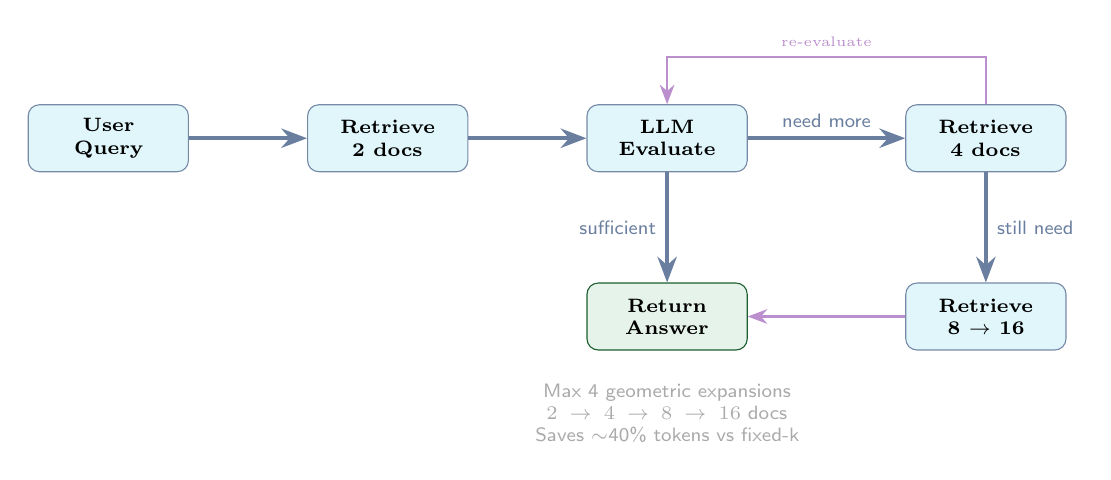
\begin{tikzpicture}[node distance=1.0cm and 1.5cm]

  \node[nlqnode] (q) {User\\Query};
  \node[nlqnode, right=1.5cm of q] (r2) {Retrieve\\2 docs};
  \node[nlqnode, right=1.5cm of r2] (eval) {LLM\\Evaluate};
  \node[nlqio,   below=1.4cm of eval] (ans) {Return\\Answer};
  \node[nlqnode, right=2.0cm of eval] (r4) {Retrieve\\4 docs};
  \node[nlqnode, below=1.4cm of r4]   (r8) {Retrieve\\8 $\to$ 16};

  % Main flow
  \draw[mainarrow] (q)    -- (r2);
  \draw[mainarrow] (r2)   -- (eval);

  % Sufficient: go down to answer
  \draw[mainarrow] (eval.south) -- node[left,font=\scriptsize\color{darkgreen}]
    {\textsf{sufficient}} (ans.north);

  % Need more: go right to retrieve 4
  \draw[mainarrow] (eval.east) -- node[above,font=\scriptsize\color{orange}]
    {\textsf{need more}} (r4.west);

  % Retrieve 4 loops back to eval
  \draw[subarrow, color=purple!60] (r4.north) -- ++(0,0.6) -| node[above,pos=0.25,font=\tiny\color{purple!60}]
    {re-evaluate} (eval.north);

  % Retrieve 4 goes to 8 if still insufficient
  \draw[mainarrow] (r4.south) -- node[right,font=\scriptsize\color{orange}]
    {\textsf{still need}} (r8.north);

  % Retrieve 8 loops back to eval
  \draw[subarrow, color=purple!60] (r8.west) -- ++(-1.2,0) |- (ans.east);

  % Caption
  \node[below=0.3cm of ans, font=\scriptsize\sffamily\color{mgray}, text width=4cm, align=center]
    {Max 4 geometric expansions\\$2 \to 4 \to 8 \to 16$ docs\\Saves $\sim$40\% tokens vs fixed-k};

\end{tikzpicture}
\end{figure}

\begin{lstlisting}[language=Python, caption={Adaptive RAG Configuration}]
from pathway.xpacks.llm.question_answering import AdaptiveRAGQuestionAnswerer
from pathway.xpacks.llm.document_store import DocumentStore

document_store = DocumentStore(
    docs=pw.io.fs.read(path="data/articles", format="binary"),
    splitter=splitters.TokenCountSplitter(max_tokens=400),
    retriever_factory=pw.indexing.UsearchKnnFactory(
        embedder=embedders.SentenceTransformerEmbedder("all-MiniLM-L6-v2"),
        metric=pw.indexing.USearchMetricKind.COS))

question_answerer = AdaptiveRAGQuestionAnswerer(
    llm=llms.LiteLLMChat(model="openrouter/google/gemma-3n-e2b-it:free"),
    indexer=document_store,
    n_starting_documents=2, factor=2, max_iterations=4)
\end{lstlisting}

\subsection{Fallback Strategy}

When \texttt{ENABLE\_PATHWAY=false} (default for quick setup), the system uses a
synchronous \texttt{RAGPipeline} backed by ChromaDB with in-memory embeddings.
All API endpoints behave identically -- only the latency profile changes.

% ============================================================
\section{Multi-Agent Reasoning System}
% ============================================================

\subsection{Overview}

Every recommendation is produced by \textbf{13 specialist agents} running in parallel.
Each agent is a LangChain chain with a narrow, well-defined responsibility.
The Decision Agent receives all outputs and synthesizes a final signal.

\subsection{Agent Architecture}

\begin{figure}[H]
\centering
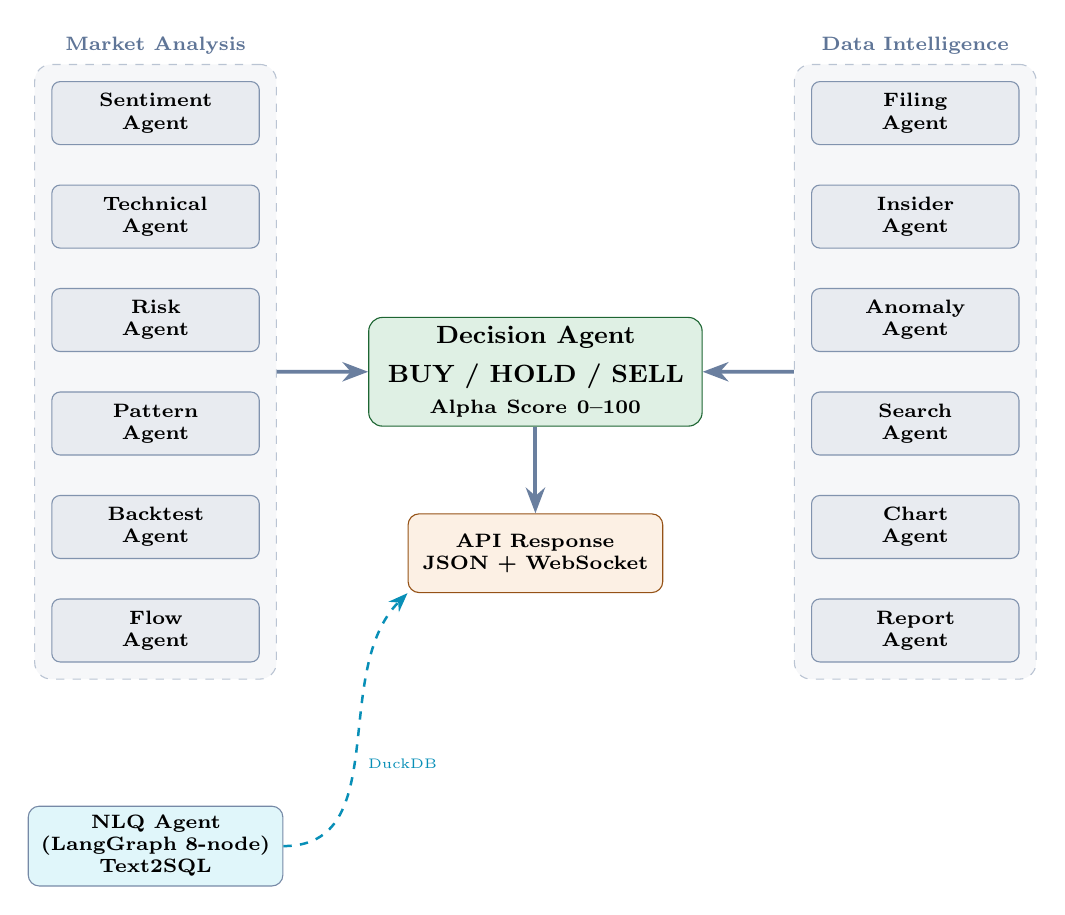
\begin{tikzpicture}[node distance=0.55cm and 0.7cm]

  %% Left column: Market Analysis
  \node[agentbox] (sentiment) {Sentiment\\Agent};
  \node[agentbox, below=0.5cm of sentiment] (technical) {Technical\\Agent};
  \node[agentbox, below=0.5cm of technical] (risk) {Risk\\Agent};
  \node[agentbox, below=0.5cm of risk] (pattern) {Pattern\\Agent};
  \node[agentbox, below=0.5cm of pattern] (backtest) {Backtest\\Agent};
  \node[agentbox, below=0.5cm of backtest] (flow) {Flow\\Agent};

  %% Right column: Data Intelligence
  \node[agentbox, right=7.0cm of sentiment] (filing) {Filing\\Agent};
  \node[agentbox, below=0.5cm of filing] (insider) {Insider\\Agent};
  \node[agentbox, below=0.5cm of insider] (anomaly) {Anomaly\\Agent};
  \node[agentbox, below=0.5cm of anomaly] (search) {Search\\Agent};
  \node[agentbox, below=0.5cm of search] (chart) {Chart\\Agent};
  \node[agentbox, below=0.5cm of chart] (report) {Report\\Agent};

  %% Group fit boxes
  \begin{pgfonlayer}{background}
    \node[groupfit, fit=(sentiment)(technical)(risk)(pattern)(backtest)(flow),
          label={[font=\scriptsize\bfseries\color{navy!70}]above:Market Analysis}] (leftgroup) {};
    \node[groupfit, fit=(filing)(insider)(anomaly)(search)(chart)(report),
          label={[font=\scriptsize\bfseries\color{navy!70}]above:Data Intelligence}] (rightgroup) {};
  \end{pgfonlayer}

  %% Decision Agent (centre)
  \node[decisionbox] (decision) at ($(leftgroup.east)!0.5!(rightgroup.west)$)
    {Decision Agent\\[3pt]{\small BUY / HOLD / SELL}\\{\scriptsize Alpha Score 0--100}};

  %% Output box
  \node[outputbox, below=1.1cm of decision] (output)
    {API Response\\JSON + WebSocket};

  %% NLQ Agent (separate)
  \node[nlqnode, below=1.6cm of leftgroup,
        text width=3.0cm, minimum width=3.2cm] (nlq)
    {NLQ Agent\\(LangGraph 8-node)\\Text2SQL};

  %% Arrows
  \draw[mainarrow] (leftgroup.east)  -- (decision.west);
  \draw[mainarrow] (rightgroup.west) -- (decision.east);
  \draw[mainarrow] (decision.south) -- (output.north);
  \draw[sidarrow] (nlq.east) to[out=0,in=225]
      node[below right,font=\tiny\color{mgray}]{DuckDB} (output.south west);

\end{tikzpicture}
\caption{13-Agent Multi-Agent Reasoning System with Alpha Score Fusion}
\end{figure}

\subsection{Agent Specifications}

\begin{center}
\scriptsize
\begin{tabular}{L{2.0cm} L{2.6cm} L{3.0cm} L{2.8cm} L{2.4cm}}
  \toprule
  \textbf{Agent} & \textbf{Input} & \textbf{Output} & \textbf{Technology} & \textbf{Data Source} \\
  \midrule
  Sentiment  & News articles & Score ($-1$ to $+1$), label & LangChain + Gemini & NewsAPI, RSS \\
  Technical  & NSE OHLCV     & RSI, SMA trend signals  & yfinance + numpy & NSE API \\
  Risk       & Price data    & Volatility, stop-loss   & Statistical calc & yfinance \\
  Pattern    & OHLCV (6 mo)  & 7 chart patterns & Custom detectors & yfinance \\
  Backtest   & Ticker + pattern & Win rate, Sharpe (5yr)& yfinance + stats & Historical \\
  Flow       & FII/DII data  & Net flow, streak detect & NSDL + analysis & NSDL \\
  Filing     & BSE annc.     & Materiality, impact     & BSE API + Gemini & BSE API \\
  Insider    & SAST/PIT data & Cluster buy/sell        & NSE + Gemini & NSE SAST \\
  Anomaly    & OHLCV series  & Anomaly flags + scores  & River ML (HST) & yfinance \\
  Search     & NLQ query     & Web search results    & LangGraph cyclic & DuckDuckGo \\
  Chart      & Ticker + events & PNG chart image       & Matplotlib & yfinance \\
  Report     & All outputs   & PDF report              & ReportLab & All agents \\
  Decision   & All agents    & BUY/HOLD/SELL + Alpha & LangChain + Gemini & All agents \\
  \bottomrule
\end{tabular}
\end{center}

\subsection{Signal Types Detected}

\begin{center}
\small
\begin{tabular}{L{3.5cm} L{3.5cm} C{2cm} C{2.5cm}}
  \toprule
  \textbf{Signal} & \textbf{Detection Method} & \textbf{Win Rate} & \textbf{Avg 30d Return} \\
  \midrule
  RSI Divergence      & Price/RSI divergence scan & 60--78\% & +3.26\% \\
  MACD Crossover      & Signal line cross + histogram & 45--57\% & +0.71\% \\
  Bollinger Breakout  & Squeeze $\to$ expansion & 55--65\% & +2.1\% \\
  Volume Breakout     & $>$2x 20-day average & 50--60\% & +1.8\% \\
  Golden Cross        & 50 SMA $>$ 200 SMA & 65--75\% & +4.2\% \\
  Insider Cluster     & 3+ insiders in 30 days & High & Varies \\
  FII Buying Streak   & 5+ consecutive sessions & $\sim$72\% & +3--5\% \\
  \bottomrule
\end{tabular}
\end{center}

\subsection{Error Handling}

\begin{center}
\small
\begin{tabular}{L{3.8cm} L{9.5cm}}
  \toprule
  \textbf{Failure Scenario} & \textbf{Recovery Strategy} \\
  \midrule
  Individual agent exception & Caught; score defaults to 0; other agents continue \\
  LLM timeout / API error & Exponential backoff $\times$ 3; falls back to rule-based score \\
  Pathway callback error & try/except in \texttt{on\_new\_article}; logs ERROR; Pathway continues \\
  DuckDB write contention & \texttt{threading.Lock} guards all writes \\
  NSE API blocked & yfinance \texttt{.NS} suffix as fallback \\
  MCP server crash & Graceful degradation -- direct DuckDB queries \\
  WebSocket disconnect & \texttt{ConnectionManager.disconnect()} removes client \\
  Missing GCP credentials & Pydantic \texttt{model\_validator} warns at startup \\
  \bottomrule
\end{tabular}
\end{center}

% ============================================================
\section{NLQ Agent Pipeline}
% ============================================================

The NLQ (Natural Language Query) system converts free-form investor questions into
SQL queries against the live DuckDB analytics database, returning \textbf{grounded, source-cited answers}.

\subsection{LangGraph 8-Node Pipeline}

\begin{figure}[H]
\centering
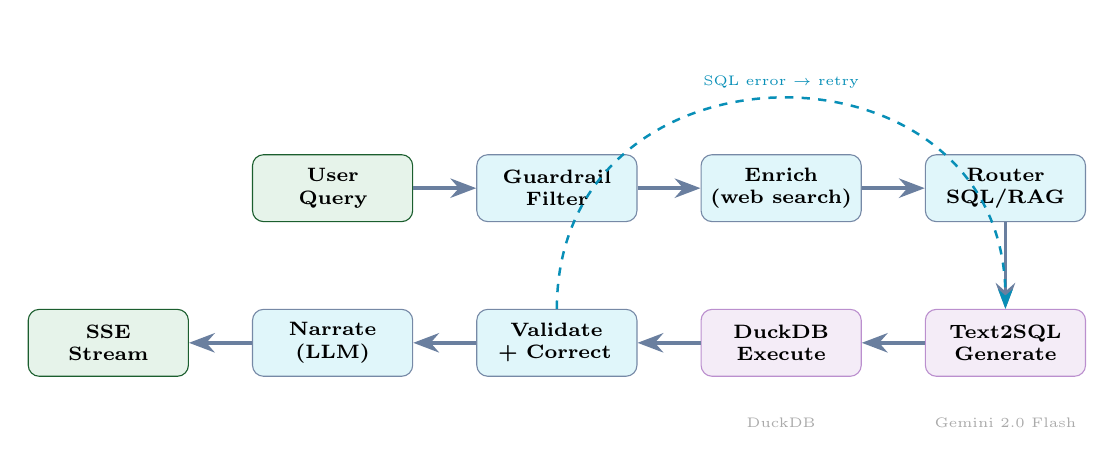
\begin{tikzpicture}[node distance=1.0cm and 0.8cm]

  \node[nlqio]   (input) {User\\Query};
  \node[nlqnode, right=0.8cm of input]  (guard)  {Guardrail\\Filter};
  \node[nlqnode, right=0.8cm of guard]  (enrich) {Enrich\\(web search)};
  \node[nlqnode, right=0.8cm of enrich] (route)  {Router\\SQL/RAG};

  \node[nlqdb,   below=1.1cm of route]  (sql)    {Text2SQL\\Generate};
  \node[nlqdb,   left=0.8cm of sql]     (exec)   {DuckDB\\Execute};
  \node[nlqnode, left=0.8cm of exec]    (valid)  {Validate\\+ Correct};
  \node[nlqnode, left=0.8cm of valid]   (narrate){Narrate\\(LLM)};
  \node[nlqio,   left=0.8cm of narrate] (out)    {SSE\\Stream};

  \draw[mainarrow] (input) -- (guard);
  \draw[mainarrow] (guard) -- (enrich);
  \draw[mainarrow] (enrich) -- (route);
  \draw[mainarrow] (route.south) -- (sql.north);
  \draw[mainarrow] (sql)    -- (exec);
  \draw[mainarrow] (exec)   -- (valid);
  \draw[mainarrow] (valid)  -- (narrate);
  \draw[mainarrow] (narrate) -- (out);

  \draw[sidarrow] (valid.north) to[out=90,in=90,looseness=1.6]
      node[above,font=\tiny\color{orange}]{SQL error $\to$ retry} (sql.north);

  \node[below=0.4cm of sql,  font=\tiny\color{mgray}] {Gemini 2.0 Flash};
  \node[below=0.4cm of exec, font=\tiny\color{mgray}] {DuckDB};

\end{tikzpicture}
\caption{LangGraph 8-Node NLQ Pipeline with SQL Correction Loop}
\end{figure}

\begin{center}
\small
\begin{tabular}{C{0.5cm} L{2.5cm} L{10cm}}
  \toprule
  \textbf{\#} & \textbf{Node} & \textbf{Responsibility} \\
  \midrule
  1 & Input Guardrail   & Rejects off-topic/harmful queries; detects PII (emails, phones), injection patterns \\
  2 & Enrichment        & Optional web search for context not in DB (recent events, company background) \\
  3 & Router            & Classifies: analytics / kpi\_lookup / portfolio / off\_topic \\
  4 & Text2SQL          & Schema linking $\to$ query planning $\to$ SQL generation via Gemini 2.0 Flash \\
  5 & DuckDB Execute    & Runs query; captures result set or error (30s timeout, 5000-row cap) \\
  6 & Validate + Correct& Checks for empty sets, type errors; retries with error context (max 2) \\
  7 & Narrate           & Converts tabular result into natural-language answer with sources \\
  8 & Output Guardrail  & Tech name redaction (``DuckDB'' $\to$ ``our analytics engine''), PII scrubbing \\
  \bottomrule
\end{tabular}
\end{center}

\subsection{MCP Servers (Model Context Protocol)}

Four MCP tool servers extend the NLQ agent's capabilities:

\begin{center}
\small
\begin{tabular}{L{3.5cm} L{9.8cm}}
  \toprule
  \textbf{MCP Server} & \textbf{Tools Provided} \\
  \midrule
  \texttt{market\_data\_server} & \texttt{get\_stock\_quote()}, \texttt{get\_latest\_signals()}, \texttt{get\_insider\_activity()}, \texttt{get\_fii\_dii\_summary()} \\
  \texttt{signal\_server} & \texttt{search\_signals\_by\_type()}, \texttt{get\_signal\_definition()}, \texttt{backtest\_signal()} \\
  \texttt{portfolio\_server} & \texttt{get\_portfolio()}, \texttt{compute\_portfolio\_return()} \\
  \texttt{search\_server} & \texttt{web\_search()}, \texttt{search\_news()} \\
  \bottomrule
\end{tabular}
\end{center}

% ============================================================
\section{WorldMonitor Global Intelligence}
% ============================================================

India's markets do not trade in isolation. AlphaStream integrates \textbf{WorldMonitor},
a global intelligence backbone, to provide cross-market context for every recommendation.

\subsection{Global Data Feeds}

\begin{center}
\small
\begin{tabular}{L{3cm} L{4.5cm} L{5.8cm}}
  \toprule
  \textbf{Category} & \textbf{Instruments} & \textbf{India Impact} \\
  \midrule
  Global Indices & NIFTY, SENSEX, S\&P 500, DOW, NASDAQ, FTSE & Correlation-based risk assessment \\
  Crypto         & BTC, ETH, SOL, XRP & Risk appetite proxy \\
  Commodities    & Gold, Crude Oil, Silver, Copper & Import cost impact on Indian cos \\
  Currencies     & INR/USD, DXY, EUR/USD & FX exposure for IT/Pharma \\
  Fear \& Greed  & CNN Fear \& Greed Index & Market sentiment gauge \\
  Macro Signals  & FRED: CPI, Yield Curve, Unemployment & Global recession risk \\
  Geopolitical   & India-focused geo-risk score & Border tensions, trade policy risk \\
  VIX            & CBOE Volatility Index & Global volatility regime \\
  \bottomrule
\end{tabular}
\end{center}

\begin{figure}[H]
\centering
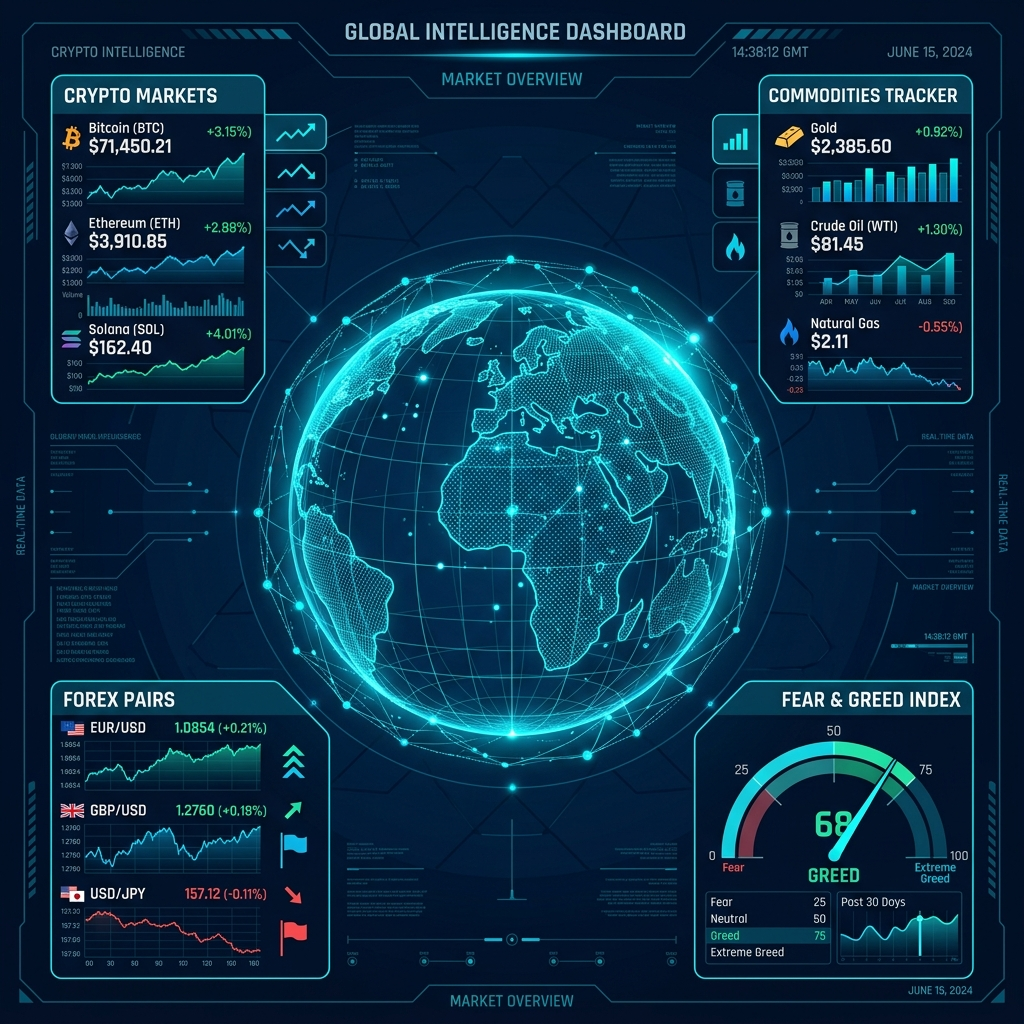
\includegraphics[width=1\textwidth]{worldmonitor_dashboard.png}
\caption{AlphaStream WorldMonitor Global Intelligence Dashboard}
\label{fig:worldmonitor}
\end{figure}

\subsection{Integration Architecture}

The \texttt{global\_market\_connector.py} reads WorldMonitor's shared JSON configurations
(\texttt{stocks.json}, \texttt{commodities.json}, \texttt{sectors.json}) and fetches live data
via yfinance and external APIs. Global signals are injected into the Decision Agent's context,
enabling India-aware global reasoning: e.g., ``Crude oil up 5\% $\to$ OMCs like BPCL/IOC under pressure.''

Nine dedicated API endpoints (\texttt{/api/global/*}) serve global data to the frontend's
\textbf{Global Intel tab}, which features a Bloomberg-style ticker tape, sector heatmaps,
Fear \& Greed gauge, and macro signal panels.

% ============================================================
\section{Technology Stack}
% ============================================================

\subsection{Backend}

\begin{center}
\small
\begin{tabular}{L{3cm} L{3.6cm} L{6.6cm}}
  \toprule
  \textbf{Component} & \textbf{Technology} & \textbf{Role} \\
  \midrule
  Streaming Engine  & Pathway            & Real-time RAG, $<$2s latency \\
  Web Framework     & FastAPI + WS + SSE & REST + real-time push \\
  LLM               & Gemini 2.0 Flash   & All agent reasoning (Vertex AI) \\
  Agent Framework   & LangChain + LangGraph & Multi-agent orchestration + NLQ \\
  Analytics DB      & DuckDB             & Pre-aggregated views, screener, Text2SQL \\
  Vector Search     & ChromaDB           & Embedding-based article retrieval \\
  Anomaly Detection & River ML (HST)     & Online price/volume anomalies \\
  Indian Data       & NSE, BSE, Groww, NSDL & OHLCV, filings, FII/DII, fundamentals \\
  Global Data       & WorldMonitor, FRED & Indices, crypto, FX, macro \\
  Package Manager   & uv                 & Fast, reproducible dependencies \\
  \bottomrule
\end{tabular}
\end{center}

\subsection{Frontend}

\begin{center}
\small
\begin{tabular}{L{3cm} L{3.6cm} L{6.6cm}}
  \toprule
  \textbf{Component} & \textbf{Technology} & \textbf{Role} \\
  \midrule
  Framework     & React 19                & UI framework \\
  Build Tool    & Vite 6                  & Dev server + bundling \\
  Styling       & Tailwind CSS 4          & Utility-first CSS \\
  Components    & shadcn/ui               & Accessible UI primitives \\
  State         & Zustand (persisted)     & Client state + localStorage \\
  Candlesticks  & lightweight-charts 5.1  & TradingView-style charting \\
  Data Charts   & Recharts 3.6            & Bar, Pie, Radar, Line charts \\
  Icons         & Lucide React            & Consistent iconography \\
  \bottomrule
\end{tabular}
\end{center}

% ============================================================
\section{API Reference}
% ============================================================

\subsection{Market Intelligence (15 endpoints)}

\begin{center}
\scriptsize
\begin{tabular}{L{5.2cm} C{1.2cm} L{6.8cm}}
  \toprule
  \textbf{Endpoint} & \textbf{Method} & \textbf{Description} \\
  \midrule
  \texttt{/api/ohlcv/\{ticker\}}           & GET  & Candlestick + optional RSI/SMA \\
  \texttt{/api/fundamentals/\{ticker\}}    & GET  & PE, PB, ROE, Div Yield, 52w H/L \\
  \texttt{/api/radar}                      & GET  & Top signals by Alpha Score \\
  \texttt{/api/screener}                   & GET  & Filter Nifty 50 (DuckDB view) \\
  \texttt{/api/patterns/\{ticker\}}        & GET  & Chart pattern detection \\
  \texttt{/api/backtest/\{ticker\}/\{pat\}}& GET  & Historical backtest (5-year) \\
  \texttt{/api/flows}                      & GET  & FII/DII flows + streak detection \\
  \texttt{/api/anomalies/\{ticker\}}       & GET  & River ML anomaly scores \\
  \texttt{/api/filings/\{ticker\}}         & GET  & BSE corporate announcements \\
  \texttt{/api/tickers}                    & GET  & Nifty 50 universe \\
  \texttt{/api/tickers/popular}            & GET  & Top 10 by market cap \\
  \texttt{/api/news}                       & GET  & Recent articles from DuckDB \\
  \texttt{/api/portfolio}                  & POST & Set user portfolio holdings \\
  \texttt{/api/portfolio/summary}          & GET  & Live P\&L summary \\
  \texttt{/api/insights}                   & GET  & Ambient AI alerts \\
  \bottomrule
\end{tabular}
\end{center}

\subsection{Global Market (9 endpoints)}

\begin{center}
\scriptsize
\begin{tabular}{L{5.2cm} C{1.2cm} L{6.8cm}}
  \toprule
  \textbf{Endpoint} & \textbf{Method} & \textbf{Description} \\
  \midrule
  \texttt{/api/global/indices}    & GET & NIFTY, SENSEX, S\&P 500, DOW, NASDAQ \\
  \texttt{/api/global/commodities}& GET & Gold, Crude Oil, Silver, Copper \\
  \texttt{/api/global/crypto}     & GET & BTC, ETH, SOL, XRP \\
  \texttt{/api/global/currencies} & GET & INR/USD, DXY, EUR/USD \\
  \texttt{/api/global/sectors}    & GET & 12 US sector ETF returns \\
  \texttt{/api/global/fear-greed} & GET & CNN Fear \& Greed index \\
  \texttt{/api/global/macro}      & GET & FRED macro signals + verdict \\
  \texttt{/api/global/vix}        & GET & VIX volatility index \\
  \texttt{/api/global/geo-risk}   & GET & India geopolitical risk score \\
  \bottomrule
\end{tabular}
\end{center}

\subsection{Core + Streaming (6 endpoints)}

\begin{center}
\scriptsize
\begin{tabular}{L{5.2cm} C{1.2cm} L{6.8cm}}
  \toprule
  \textbf{Endpoint} & \textbf{Method} & \textbf{Description} \\
  \midrule
  \texttt{/recommend}             & POST     & Full 13-agent recommendation \\
  \texttt{/api/nlq}               & POST     & NLQ blocking response \\
  \texttt{/api/nlq/stream}        & POST/GET & NLQ with SSE streaming \\
  \texttt{/insider/\{ticker\}}    & GET      & NSE SAST/PIT insider trading \\
  \texttt{/report/\{ticker\}}     & POST     & PDF report generation \\
  \texttt{/ws/stream/\{ticker\}}  & WS       & Real-time rec + market updates \\
  \bottomrule
\end{tabular}
\end{center}

% ============================================================
\section{Bloomberg-Style Terminal (Frontend)}
% ============================================================

The React 19 frontend presents a \textbf{5-tab Bloomberg-style terminal} with 25+ components:

\begin{center}
\small
\begin{tabular}{C{0.5cm} L{2.5cm} L{10cm}}
  \toprule
  \textbf{\#} & \textbf{Tab} & \textbf{Components} \\
  \midrule
  1 & Overview & TradingView candlestick chart (RSI + SMA overlays), AI Recommendation Card
      (BUY/SELL/HOLD + reasoning), Stock Fundamentals (PE, PB, ROE from Groww),
      Insider Activity, Agent Radar, Anomaly Panel \\
  2 & Signals & Stock Screener (filter Nifty 50 by sector/direction/alpha),
      Opportunity Radar (signal cards with backtest win rates), FII/DII Flow Chart,
      Sector Heatmap \\
  3 & Global Intel & Bloomberg ticker tape, Global Markets Panel (indices, crypto,
      commodities), Fear \& Greed Gauge, Macro Signal Panel (FRED),
      Commodity Strip, Geopolitical Risk Panel \\
  4 & Company & Corporate Filings (BSE, 7/30/90-day view),
      Articles List (sorted by threat level), Watchlist Panel (up to 20 tickers) \\
  5 & Portfolio & Portfolio Manager (add/remove holdings, real-time P\&L),
      History Chart, Sector Allocation PieChart \\
  \bottomrule
\end{tabular}
\end{center}

\begin{figure}[H]
\centering
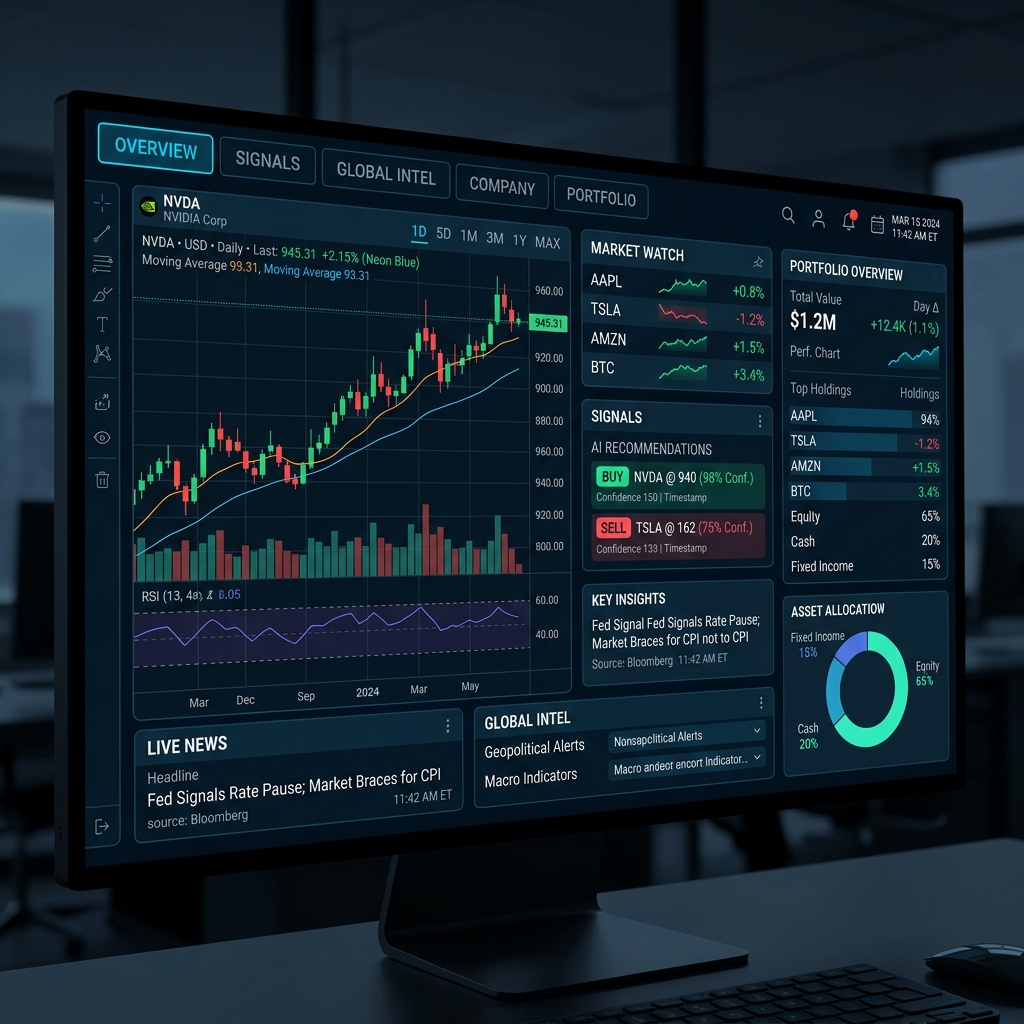
\includegraphics[width=1\textwidth]{terminal_ui_mockup.png}
\caption{AlphaStream Bloomberg-Style React 19 Frontend Terminal}
\label{fig:terminal}
\end{figure}

\noindent
The \textbf{NLQ Panel} (``Market ChatGPT Next Gen'') is accessible from any tab via a floating
button. It streams responses via SSE, shows the thought process (guardrail $\to$ route $\to$
SQL $\to$ narrate), and provides context-aware quick prompts that change based on the active tab.

% ============================================================
\section{Business Impact Model}
\label{sec:impact}
% ============================================================

\subsection{Market Sizing (TAM / SAM / SOM)}

\begin{center}
\small
\begin{tabular}{L{1.5cm} L{5cm} C{2.5cm} L{4.5cm}}
  \toprule
  \textbf{Level} & \textbf{Segment} & \textbf{Size} & \textbf{Rationale} \\
  \midrule
  \textbf{TAM} & Total Indian equity participants & 14 Cr & CDSL + NSDL demat accounts (2024) \\
  \textbf{SAM} & Active traders researching daily & $\sim$3 Cr & $\approx$20\% trade monthly \\
  \textbf{SOM} & 5-year premium capture & 1.5 L & 0.5\% of SAM (conservative) \\
  \bottomrule
\end{tabular}
\end{center}

\noindent
\small\textit{Key assumption: SOM uses 0.5\% of SAM, not TAM -- anchored to paying users, not total accounts.}

\subsection{User Impact -- Time Saved}

\begin{greenbox}[title={Time Value Recovered Per User}]
\textbf{1.75 hours/day} $\times$ \Rs{}500/hr $\times$ 250 trading days
$= \mathbf{\Rs{}2.19\ Lakh/user/year}$ in recovered productivity.
\end{greenbox}

\begin{center}
\small
\begin{tabular}{L{4cm} L{3.5cm} L{3.5cm}}
  \toprule
  \textbf{Task} & \textbf{Without AlphaStream} & \textbf{With AlphaStream} \\
  \midrule
  Daily research          & 2+ hours         & 15 minutes \\
  Filing analysis         & 30 min/filing (manual) & Instant LLM classification \\
  Insider trade monitoring& Manual NSE checks & Automated alerts \\
  FII/DII tracking        & Visit NSDL daily  & Real-time flow analysis \\
  \bottomrule
\end{tabular}
\end{center}

\subsection{User Impact -- Alpha Generated}

\begin{center}
\small
\begin{tabular}{L{3.5cm} L{3.5cm} C{2cm} C{3cm}}
  \toprule
  \textbf{Signal Type} & \textbf{Detection} & \textbf{Win Rate} & \textbf{Avg 30d Return} \\
  \midrule
  RSI Divergence      & Automated scan   & 60--78\% & +3.26\% \\
  MACD Crossover      & Real-time detect.& 45--57\% & +0.71\% \\
  Insider Cluster Buy & 3+ insiders/30d  & High (historical) & Varies \\
  FII Buying Streak   & 5+ sessions      & $\sim$72\% & +3--5\% \\
  \bottomrule
\end{tabular}
\end{center}

\begin{orangebox}[title={Conservative Alpha Estimate}]
2--3 actionable signals/month $\times$ 60\% accuracy $\times$ \Rs{}3,000 average gain
$= \mathbf{\Rs{}54,000/user/year}$ in additional alpha.
\end{orangebox}

\subsection{Risk Reduction}

\begin{itemize}[leftmargin=1.6em, itemsep=2pt]
  \item Early warning on adverse signals prevents panic selling
  \item Portfolio-aware alerts: ``Your IT holdings at risk from FII selling streak''
  \item Backtested confidence: ``This pattern has worked 78\% of the time on this stock''
  \item Estimated \textbf{15\% reduction} in behavioral losses
\end{itemize}

\subsection{ET Markets Revenue Projection}

\begin{center}
\small
\begin{tabular}{L{4.5cm} C{2.8cm} C{2.8cm} C{2.8cm}}
  \toprule
  & \textbf{Year 1} & \textbf{Year 3} & \textbf{Year 5} \\
  \midrule
  Premium users (\Rs{}999/month)  & 50,000 & 2,00,000 & 5,00,000 \\
  \textbf{Annual Revenue}     & \textbf{\Rs{}59.9 Cr} & \textbf{\Rs{}239.8 Cr} & \textbf{\Rs{}599.4 Cr} \\
  \bottomrule
\end{tabular}
\end{center}

\subsection{Cost Reduction for ET Markets}

\begin{center}
\small
\begin{tabular}{L{4cm} L{3.5cm} L{3.5cm} L{2.5cm}}
  \toprule
  \textbf{Cost Category} & \textbf{Current} & \textbf{With AlphaStream} & \textbf{Saving} \\
  \midrule
  Signal content (est.) & \Rs{}20 Cr/yr & LLM-generated, human-reviewed & \Rs{}5--10 Cr/yr \\
  & (manual analysts) & signal summaries & (30\% reduction) \\
  \bottomrule
\end{tabular}
\end{center}

\noindent
\small\textit{Automated pipelines handle high-frequency, repeatable content (FII flows, insider alerts,
technical scans). Humans focus on narrative and investigative content -- higher value, lower volume.}

\subsection{Competitive Moat}

\begin{enumerate}[leftmargin=1.8em, itemsep=3pt]
  \item \textbf{India-specific regulatory data} -- NSE SAST/PIT and NSDL FII/DII feeds
        not available through generic global APIs.
  \item \textbf{Backtested signals, not LLM speculation} -- every signal carries a win rate
        grounded in NSE/BSE historical data.
  \item \textbf{Streaming architecture} -- Pathway incremental indexing vs.\ static
        dashboards that recompute on every load.
  \item \textbf{Portfolio-aware alerts} -- signals contextualised to each user's
        actual holdings.
  \item \textbf{Compound improvement} -- each interaction improves signal ranking;
        accuracy scales with user base.
\end{enumerate}

\subsection{Assumptions (Stated Explicitly)}

\begin{enumerate}[leftmargin=1.8em, itemsep=1pt]
  \item Win rates based on backtesting against Nifty 50 stocks with 3--5 year data
  \item Average return estimates use median, not mean (to reduce outlier effect)
  \item Time savings assumes basic digital literacy and daily market participation
  \item Premium conversion rate of 0.3\% is conservative (industry average 0.5--1\%)
  \item Back-of-envelope calculations -- detailed validation would require A/B testing
  \item SOM (1.5L users) = 0.5\% of SAM (3 Cr active traders) -- conservative for 5-year horizon
  \item Revenue projections assume no price increase over 5 years (understates upside)
  \item Cost reduction estimate assumes research content budget of $\sim$\Rs{}20 Cr/year
  \item Year 3/5 projections assume compounding growth of $\sim$100\%/150\% from Year 1
\end{enumerate}

% ============================================================
\section{Demonstration \& Verification}
% ============================================================

\subsection{Live Demo Flow}

\begin{enumerate}[leftmargin=1.8em, itemsep=3pt]
  \item \textbf{Login} -- Open dashboard at \texttt{http://localhost:5173}; login as judge
  \item \textbf{Overview Tab} -- RELIANCE loads by default: candlestick chart, AI recommendation,
        fundamentals, insider activity, anomaly detection
  \item \textbf{Signals Tab} -- Stock Screener filters Nifty 50; Opportunity Radar shows top signals
  \item \textbf{Global Intel} -- Bloomberg ticker tape, crypto, FX, Fear \& Greed, macro signals
  \item \textbf{NLQ Chat} -- Ask ``Which stocks have FII buying streaks?'' -- grounded Text2SQL answer
  \item \textbf{Real-time} -- Inject breaking news via API; watch recommendation update in $<$2s
\end{enumerate}

\subsection{Expected Latencies}

\begin{center}
\small
\begin{tabular}{L{6cm} C{4cm}}
  \toprule
  \textbf{Operation} & \textbf{Latency} \\
  \midrule
  Article ingestion to DuckDB     & $<$100 ms \\
  Pathway RAG indexing            & $<$200 ms \\
  13-agent recommendation         & $\sim$1.2 s (LLM-bound) \\
  WebSocket delivery to browser   & $<$50 ms \\
  \textbf{Total: news $\to$ UI update} & \boldmath$<$\textbf{2 seconds} \\
  Adaptive RAG token savings      & $\sim$40\% vs fixed-k \\
  PDF report generation           & $\sim$15 s \\
  \bottomrule
\end{tabular}
\end{center}

% ============================================================
\section{Setup \& Quick Start}
% ============================================================

\subsection{Prerequisites}

\begin{itemize}[leftmargin=1.6em, itemsep=2pt]
  \item Python 3.11+ and \texttt{uv} package manager
  \item Node.js 18+ (frontend)
  \item Google Cloud account with Vertex AI (Gemini 2.0 Flash)
  \item \texttt{NEWS\_API\_KEY} from newsapi.org (for live news)
  \item 4 GB+ RAM recommended
\end{itemize}

\subsection{Three-Command Setup}

\begin{lstlisting}[language=bash]
# 1. Clone and install backend
git clone https://github.com/wildcraft958/AlphaStream_India.git
cd AlphaStream_India/backend
cp .env.example .env   # Add API keys
uv sync && uv run python -m src.data.market_schema

# 2. Start backend (cold start ~75s)
./start.sh   # OR: uv run uvicorn src.api.app:app --port 8000

# 3. Start frontend (new terminal)
cd ../frontend && npm install && npm run dev
# Open http://localhost:5173
\end{lstlisting}

\subsection{Key Environment Variables}

\begin{center}
\small
\begin{tabular}{L{5.5cm} L{7.8cm}}
  \toprule
  \textbf{Variable} & \textbf{Purpose} \\
  \midrule
  \texttt{\small GOOGLE\_APPLICATION\_\newline CREDENTIALS} & Path to GCP service-account JSON \\
  \texttt{GCP\_PROJECT\_ID}    & GCP project ID for Vertex AI \\
  \texttt{NEWS\_API\_KEY}      & NewsAPI key for live article ingestion \\
  \texttt{ENABLE\_PATHWAY}     & \texttt{true} = Pathway RAG; \texttt{false} = sync fallback \\
  \texttt{GROWW\_API\_TOKEN}   & Groww fundamentals (PE, PB, ROE) \\
  \texttt{FRED\_API\_KEY}      & FRED macro signals (CPI, yield curve) \\
  \bottomrule
\end{tabular}
\end{center}

% ============================================================
\section*{Appendix: Repository Structure}
% ============================================================

\begin{center}
\small
\begin{tabular}{@{}L{0.5cm} L{4.2cm} L{8.8cm}@{}}
  \toprule
  & \textbf{\sffamily\color{navy}Directory / File} & \textbf{\sffamily\color{navy}Purpose} \\
  \midrule
  \multirow{6}{*}{\rotatebox[origin=c]{90}{\scriptsize\sffamily\color{cyan!70!navy}\textbf{BACKEND}}}
  & \texttt{backend/src/agents/} & 13 AI agents (Sentiment, Technical, Risk, \ldots) + NLQ pipeline + MCP servers \\
  & \texttt{backend/src/connectors/} & Data source adapters: NSE, BSE, Groww, WorldMonitor, FII/DII \\
  & \texttt{backend/src/pipeline/} & Pathway streaming engine + Adaptive RAG + Fusion Engine \\
  & \texttt{backend/src/api/} & FastAPI application: market, NLQ, global routers \\
  & \texttt{backend/src/data/} & DuckDB schema definitions + Nifty 50 seed data \\
  & \texttt{backend/start.sh} & One-command startup (respects \texttt{ENABLE\_PATHWAY}) \\
  \midrule
  \multirow{2}{*}{\rotatebox[origin=c]{90}{\scriptsize\sffamily\color{green!70!black}\textbf{FE}}}
  & \texttt{frontend/src/components/} & 25+ Bloomberg terminal components (charts, screener, NLQ) \\
  & \texttt{frontend/src/store/} & Zustand state management + localStorage persistence \\
  \midrule
  & \texttt{worldmonitor/} & Global intelligence: 3D globe, 86 panels, 435+ news feeds \\
  \midrule
  \multirow{3}{*}{\rotatebox[origin=c]{90}{\scriptsize\sffamily\color{purple!80}\textbf{DOCS}}}
  & \texttt{docs/*.png} & Architecture diagrams (system, agents, herd-of-knowledge) \\
  & \texttt{docs/impact\_model.md} & TAM/SAM/SOM + revenue projections \\
  & \texttt{docs/submission.tex} & This document (LaTeX source) \\
  \midrule
  & \texttt{demo\_pipeline.py} & 8-step automated demo with JSON proof generation \\
  & \texttt{README.md} & Project overview + full API reference (24 endpoints) \\
  \bottomrule
\end{tabular}
\end{center}

\begin{center}
  \small\sffamily\color{steel}Full source: \url{https://github.com/wildcraft958/AlphaStream_India}
\end{center}

\vfill
\begin{center}
  {\color{cyan}\rule{0.6\linewidth}{0.8pt}}\\[4pt]
  {\small\color{mgray}AlphaStream India \textbullet{} ET AI Hackathon 2026 \textbullet{}
   Problem Statement 6: AI for the Indian Investor}\\[2pt]
  {\small\color{navy}\url{https://github.com/wildcraft958/AlphaStream_India}}
\end{center}

\end{document}
